\chapter{자기주도적 학습 과제 6 (14.4-5)}
\section{함수가 가진 변수의 개수에 상관 없이 하나의 식으로 연쇄법칙을 나타낼 수 있을까요}
실은 하나의 식이라고 생각한다. 그냥 모든 변수에 대해 미분한 어떤 식이 있을 수 있고,

적당히, 독립인 변수들은 서로의 미분이 0임을 넣어 주면 될 것 같다.

\section{방향도함수의 정의와 기하학적 의미}
점 $p=(x_0, y_0)$에서 $u$ 방향의 방향미분계수는 다음과 같이 정의된다.

$$(D_u f)_p = \lim_{h \to 0} \frac{f(p+hu) - f(p)}{h}$$
이 값을 갖는 함수를 방향도함수로 정의한다.

이 값은, 어떤 함수를 $p$와 평행하게 자른 단면에서의 기울기를 나타내는 것이다.

\section{기울기 연산의 정의과 기하학적 의미}
점 $p=(x_0, y_0)$에서 $f$를 기울기 연산한 것은 다음과 같이 정의한다.
$$\nabla f  = \frac{\partial f}{\partial x}i + \frac{\partial f}{\partial y}j$$

이는, $f$가 증가하는 방향을 나타낸다.
\section{$f: \mathbb{R}^2 \to \mathbb{R}$이고, 0에서 모든 방향의 방향미분계수 갖으며, 0에서만 불연속 함수찾기}
$f(0,0)=0$으로 정의하자. 0에서 연속 아니지만 미분방향계수 존재하는 '그' 문제 생각. 그 문제에서 불연속적인 부분을 깍아서 매끄럽게(?) 만들면 되지 않을까 생각.
$$f(x,y) = \begin{cases}
    e^{\left|\frac{x-y^2}{y^3} \right|} & y \ne 0\\
    0, & y = 0
\end{cases}
$$


\begin{figure}[h!]
    \centering
    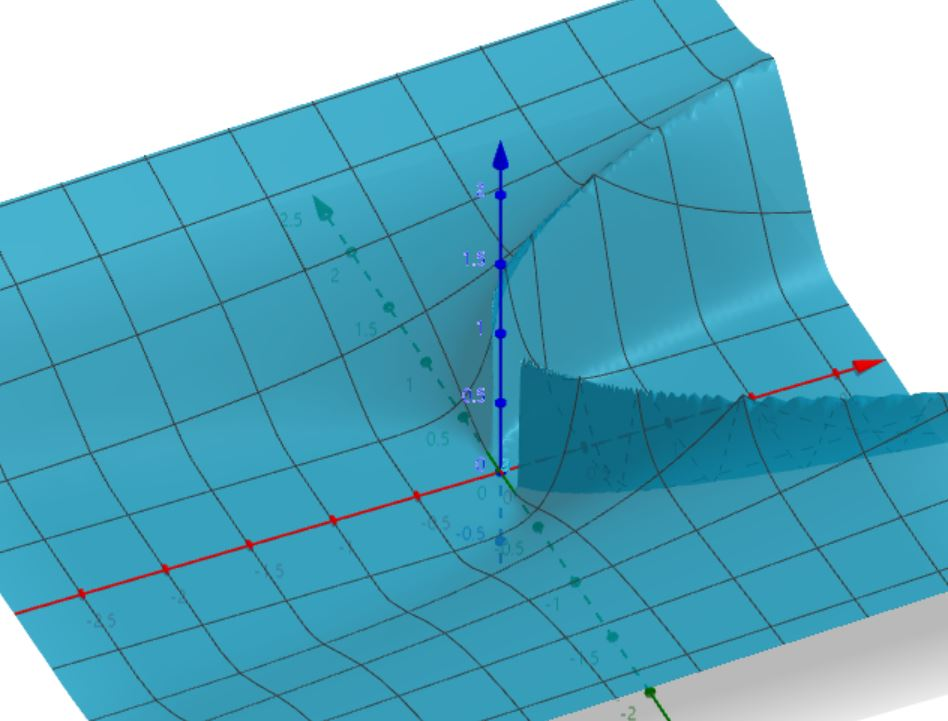
\includegraphics[width=.7\textwidth]{img/strange.JPG  }
    \caption{대충 이렇게 생김}
    \label{texlive:exdit}
\end{figure}
\paragraph{증명}
$u=(0,1)$에 대하여,
$$lim_{h \to 0} \frac{f(0,0)-f(h,kh)}{h} = lim_{h \to 0} \frac{e^{-1/|h|}}{h} = 0$$

$u=(1,k)$에 대하여는, '그'문제 증명하듯이 증명하면 됨.

하지만, $x=y^2$라면, $f(x,y)=1$이므로, 안됨,


\section{복소함수의 미분과 편미분}
미분은 똑같이 정의한다.
$$f'(z) = \lim_{\Delta z \to 0} \frac{f(z_0 + \Delta z) -f(z_0)}{\Delta z}$$
실수축과 허수축에 대해 편미분(?) 할 수 있는 것 같다.
